\documentclass{standalone}
\usepackage{xcolor}
\usepackage{verbatim}
\usepackage{tikz}
\usepackage[T1]{fontenc}
\usepackage{graphics}
\usepackage{hyperref}
\newcommand{\code}[1]{\texttt{#1}}
\newcommand{\R}{R}
\newcommand{\pkg}[1]{#1}
\newcommand{\CRANpkg}[1]{\pkg{#1}}%
\newcommand{\BIOpkg}[1]{\pkg{#1}}
\usetikzlibrary{snakes,shapes,backgrounds,arrows}
\begin{document}
\nopagecolor
\tikzset{
  state/.style={circle,draw,minimum size=10ex},
  arrow/.style={-latex}}
\centering
\tikzset{
  state/.style={circle,draw,minimum size=10ex},
  arrow/.style={-latex}}
 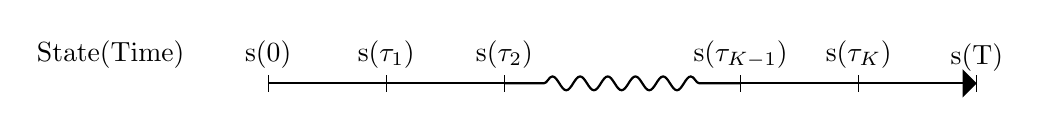
\begin{tikzpicture}[snake=snake, line before snake = 5mm, line after snake = 5mm]
    % draw horizontal line
    \draw[thick] (-2,.8) -- (1,.8);
     \draw[snake,thick] (1,.8) -- (4,.8);
  \draw[-triangle 90,thick]  (4,.8) -- (7,.8);
    % draw vertical lines
    \foreach \x in {-2,-.5,1,4,5.5,7}
      \draw (\x cm,.8cm+3pt) -- (\x cm,.8cm-3pt);
    % draw nodes
    \draw (-2,1.5) node[below=1pt] { s(0) } ;
    \draw (-.5,1.5) node[below=1pt] { s($\tau_1$) } ;
    \draw (1,1.5) node[below=1pt] { s($\tau_2$) };
     \draw (4,1.5) node[below=1pt] {s($\tau_{K-1}$)};
    \draw (5.5,1.5) node[below=1pt] {s($\tau_{K}$)};
    \draw (7,1.5) node[below=2pt] {s(T)};
  %  \draw (-5,0) node[above=3pt] { Time };
    \draw (-4,1.5) node[below=1pt] {State(Time)} ;
  \end{tikzpicture}
\end{document}
